\documentclass[a4paper]{article}
%\usepackage[T1]{fontenc}
\usepackage[english]{babel}

\usepackage{amsmath}
\usepackage{amssymb,amsfonts,textcomp, graphicx}
\usepackage{graphics}

\usepackage{wrapfig}

\usepackage{parskip}

\usepackage{color}
\usepackage{array}
\usepackage{hhline}
\usepackage{subcaption}

\usepackage{textcomp}

\usepackage[hidelinks]{hyperref}

\setlength\tabcolsep{1mm}
\renewcommand\arraystretch{1.3}

\setlength\voffset{-1in}
\setlength\hoffset{-1in}
\setlength\topmargin{0.7874in}
\setlength\oddsidemargin{0.7874in}
\setlength\textheight{10.118099in}
\setlength\textwidth{6.6932993in}
\setlength\footskip{0.0cm}
\setlength\headheight{0cm}
\setlength\headsep{0cm}


\begin{document}

\newcommand\textstyleEmphasis[1]{\textit{#1}}
\renewcommand{\contentsname}{Table des mati\`eres}
\renewcommand\refname{R\'ef\'erences}

\renewcommand{\abstractname}{Pr\'eambule}
\title{\textbf{Projet Circuits Int\'egr\'es Radiofr\'equence \\ TP Adaptation en Puissance}}
\author{Mohamed Hage Hassan \\ Cl\'ement Cheung}
\date{6 D\'ecembre 2017}
\maketitle
\thispagestyle{empty}


\iffalse
\clearpage
\fi

\tableofcontents
\clearpage

\iffalse

\begin{figure}[!htb]
\begin{center}
  \includegraphics[scale=0.47]{Echantillonneur-bloqueur.png}
  \caption{Sch\'ema d'un \'echantilloneur-bloqueur \`a capacit\'e commut\'ee}
\end{center}
\end{figure}

\fi

\section*{Introduction}
\addcontentsline{toc}{section}{Introduction}

\section{Imp\'edance et Admittance - Analyse sous Cadence}
\subsection{\'Etude th\'eorique}

On essaye en premier temps de retrouver le circuit \'equivalent au celui RC en s\'erie :
On a :
\begin{equation}
  Z_C = \frac{1}{jC\omega} \phantom{8} \phantom{8} \phantom{8} X_S = - \frac{1}{C\omega}j
\end{equation}

Sachant que :
\[
Q = \frac{\|X_S \|}{R} = \frac{1}{R_S C\omega} = 0.159 < 3
\]
\[
X_S = \frac{1}{C_S \omega} = 159.15
\]

On prend :
\begin{equation}
  \begin{split}
  R_p = R_S (1 + Q^2) \\
  X_p = X_S \frac{(1+Q^2)}{Q^2}
  \end{split}
\end{equation}

Ce qui nous donne $R_p = 1025,28 \Omega$, $X_p = 6.454 \times 10^3$
\[
X_P = \frac{1}{C_P \omega} \implies C_P = \frac{1}{X_P \omega} = 24.7 fF
\]

\subsection{Simulation sous Cadence}
\textcolor{red}{\textbf{Que repr\'esente $S_{11}$?}}\\
On effectue une simulation du circuit RC pour analyser les param\`etres $S_{11}$, $Z_{11}$ et $Y_{11}$

\begin{figure}[!htb]
  \begin{subfigure}[t]{.5\linewidth}
      \centering
      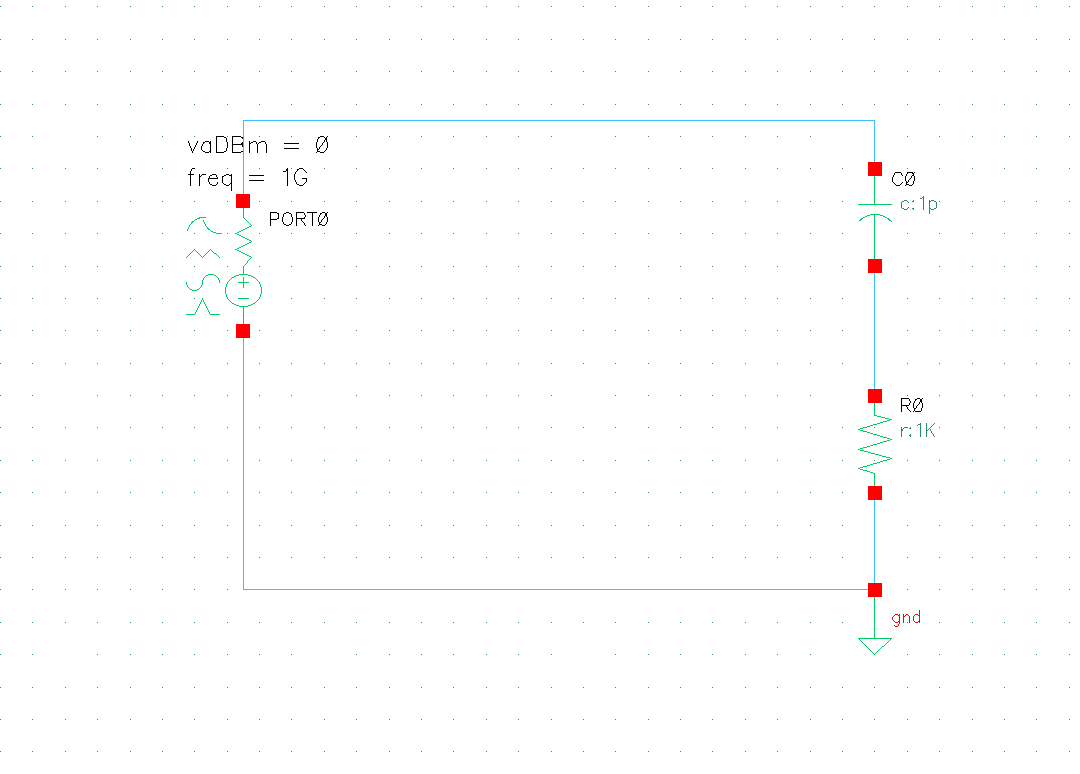
\includegraphics[width=1.1\linewidth]{circuit-RC.png}
      \label{fig:rccircuit}
  \end{subfigure}%
  \begin{subfigure}[t]{.5\linewidth}
    \centering
    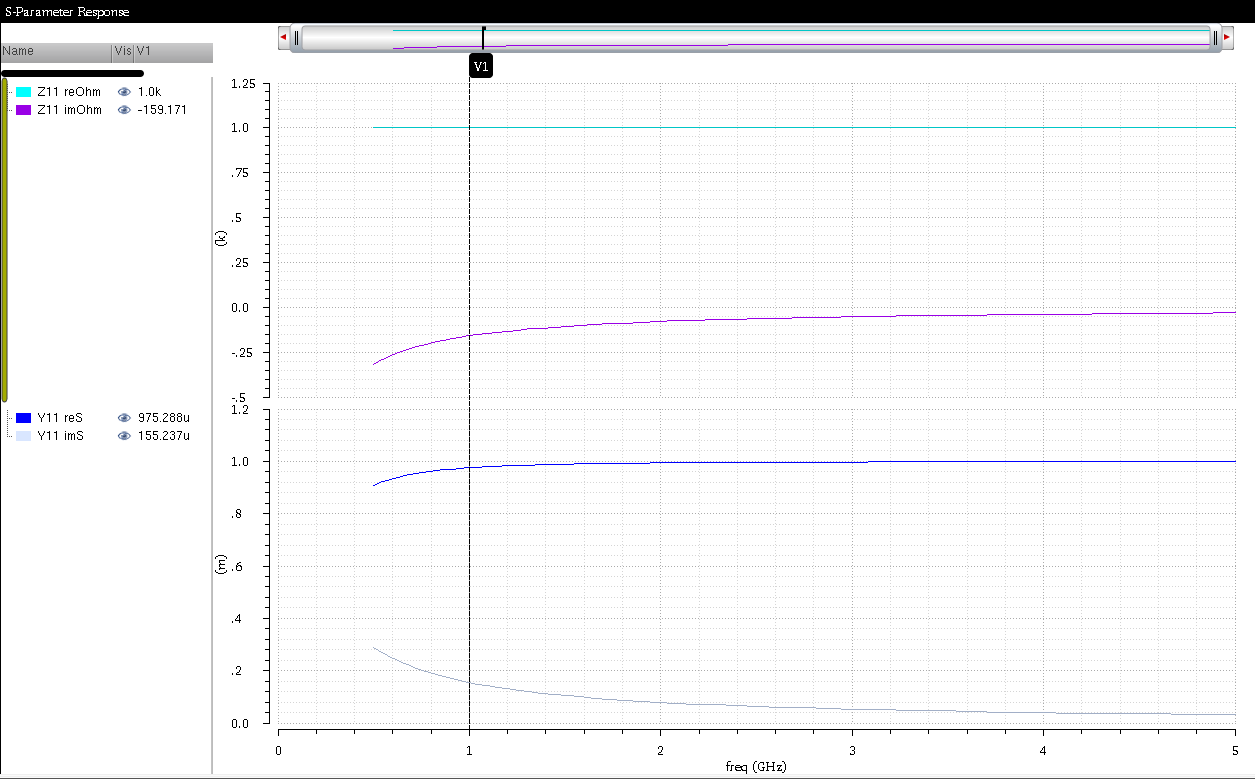
\includegraphics[width=1.1\linewidth]{sim-inital.png}
    \label{fig:rccircuit-sim}
  \end{subfigure}%
  \caption{Sch\'ema et Simulation du circuit}
  \label{fig:RC-sim}
\end{figure}

\clearpage

On retrouve :
\begin{equation}
  \begin{split}
    S_{11} = 0.906911 - j 0.0141 \\
    Z_{d} = 20 - j 3.19066 \\
    Y_{d} = 0.04859 + j 0.00777
  \end{split}
\end{equation}

Sachant que $ Y = G + j B $
\[
G = \frac{1}{R_P} \implies R_p = \frac{1}{G} = 1025 \Omega
\]
\[
B = \frac{1}{X_P} \implies X_P = \frac{1}{B} = 6.442 \times 10^3
\]


\section{Adaptation \`a $Z_0$}

\subsection{Adaptation avec un transformateur d'imp\'edance}
\subsubsection{Annulation de la partie imaginaire}
On ajoute une inductance en s\'erie au circuit RC, pour annuler la partie imaginaire $X_S$.
\[
X_L = \omega L = - X_S \implies X_L = 159.15
\]
\[
L = \frac{X_L}{\omega} = 25.33 nH
\]

\begin{figure}[!htb]
  \begin{subfigure}[t]{.5\linewidth}
      \centering
      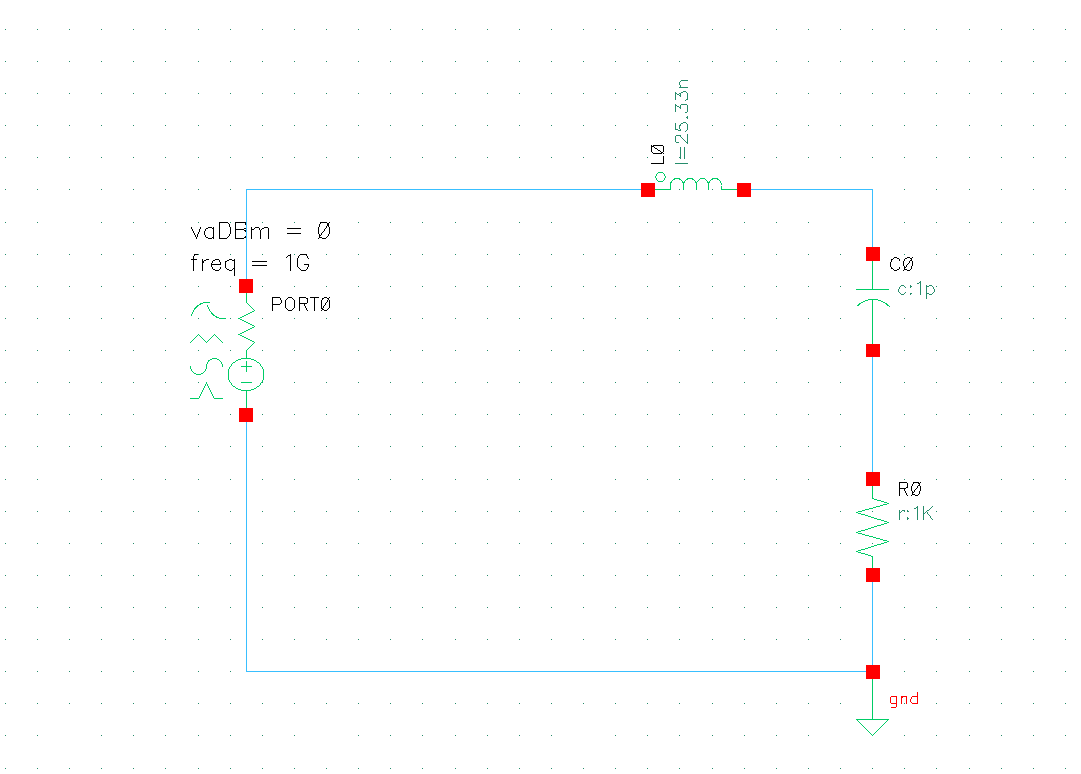
\includegraphics[width=1.1\linewidth]{circuit-LRC.png}
      \label{fig:rccircuit}
  \end{subfigure}%
  \begin{subfigure}[t]{.5\linewidth}
    \centering
    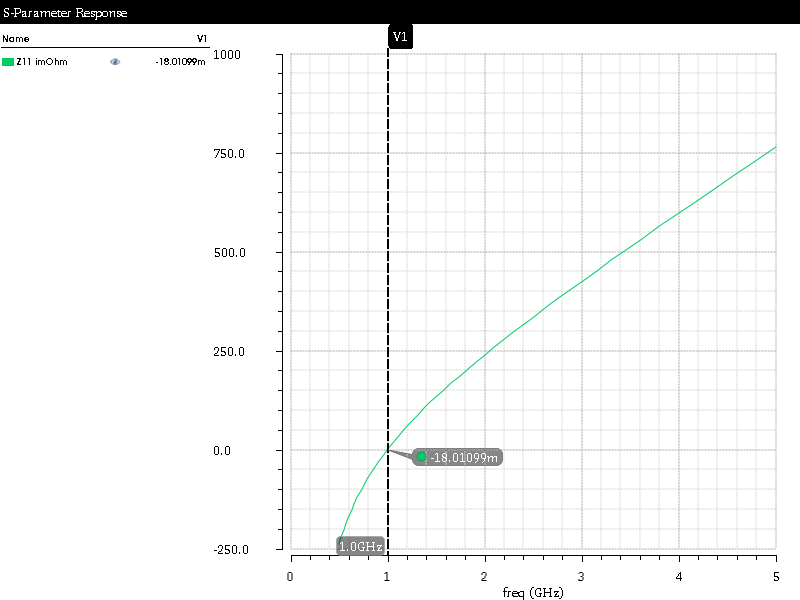
\includegraphics[width=1\linewidth]{sim-LRC.png}
    \label{fig:rccircuit-sim}
  \end{subfigure}%
  \caption{Sch\'ema et Simulation du circuit}
  \label{fig:RC-sim}
\end{figure}

\subsubsection{Abaissement de l'imp\'edance}
On ajoute une capacit\'e en parall\`ele pour abaisser la tension : \\
$Re\{Z_{in}\} = 50 \Omega$ et pour le circuit LRC, on a $Z_0 = R_0$ \`a la r\'esonance.

\[
\frac{1}{Z_{in}} =\frac{1}{Z_1} + \frac{1}{Z_0} = jC_1\omega_0 + \frac{1}{R_0}
\]

\[
Z_{in} = \frac{1}{jC_1\omega_0 + \frac{1}{R_0}}
\]

et
\[
Re\{Z_{in}\} = 50 \Omega = Re\bigg(\frac{R_0}{1+ j R_0 C_1 \omega_0}\bigg)
\]

Pour $Z_{in}$ :
\[
Z_{in} = \frac{(1 - j R_0 C_1 \omega_0) R_0}{1 + (R_0 C_1 \omega_0)^2} =\frac{R_0}{1 + (R_0 C_1 \omega_0)^2} - j \frac{R^2_0 C_1 \omega_0} {1 + (R_0 C_1 \omega_0)^2}
\]

\[
\implies R_0 C_1 \omega_0 = \sqrt{\frac{R_0}{R_e\{Z_{in}\}} - 1}
\]

\[
 C_1  = \frac{1}{R_0 \omega_0}\sqrt{\frac{R_0}{R_e\{Z_{in}\}} - 1}
\]

On retrouve $ C_1 = 693.7 fF$.

\begin{figure}[!htb]
  \begin{subfigure}[t]{.5\linewidth}
      \centering
      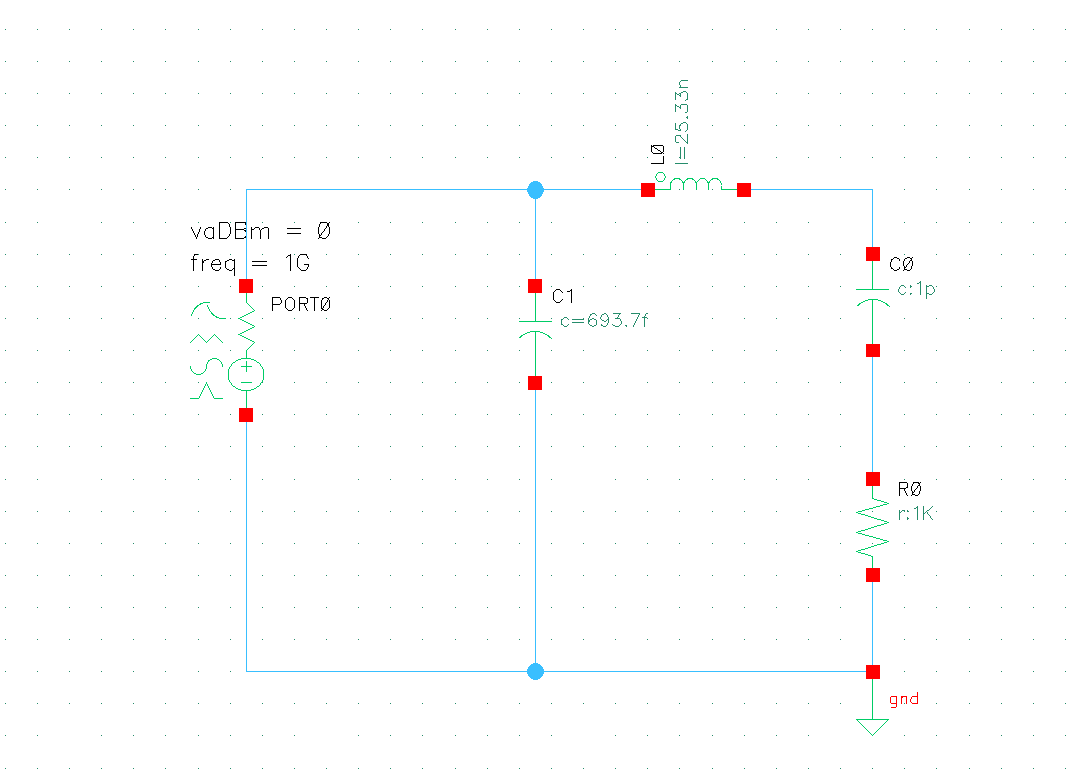
\includegraphics[width=1.1\linewidth]{Circuit-C1.png}
      \label{fig:c1circuit}
  \end{subfigure}%
  \begin{subfigure}[t]{.5\linewidth}
    \centering
    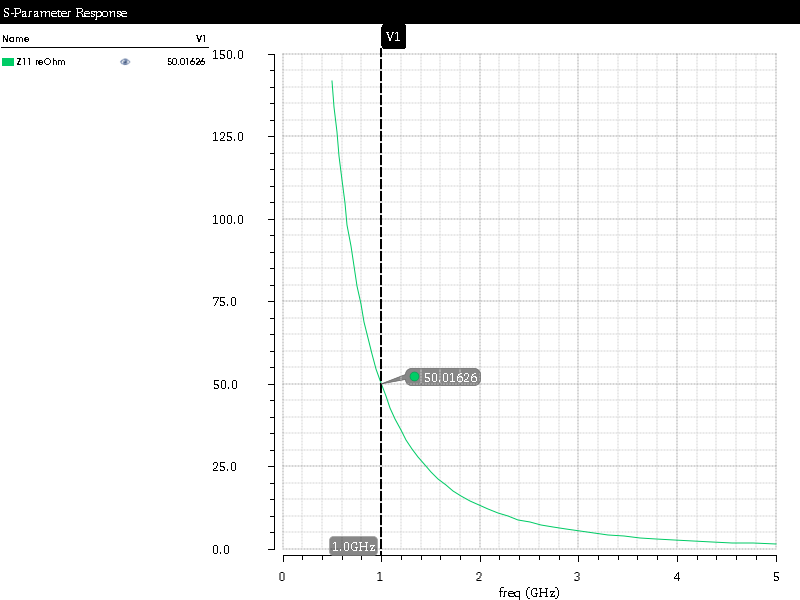
\includegraphics[width=1\linewidth]{Circuit-C1-sim.png}
    \label{fig:c1circuit-sim}
  \end{subfigure}%
  \caption{Sch\'ema et Simulation du circuit}
  \label{fig:C1-sim}
\end{figure}


\subsubsection{Adjustement final de l'imp\'edance}
On essaye d'annuler la partie imaginaire \`a l'\'entr\'ee du circuit d'adaptation : On ajoute une imp\'edance en s\'erie.
Sachant que : $X_{L1} = \omega_0 L_1$
\[
X_{L11} = - Img\{Zin\} = \frac{R^2_0 C_1 \omega_0} {1 + (R_0 C_1 \omega_0)^2}
\]
\[
\implies L_1 = \frac{R^2_0 C_1} {1 + (R_0 C_1 \omega_0)^2} \implies L_1 = 34.6 nH
\]
\begin{figure}[!htb]
  \centering
  \begin{subfigure}[t]{.4\linewidth}
      \centering
      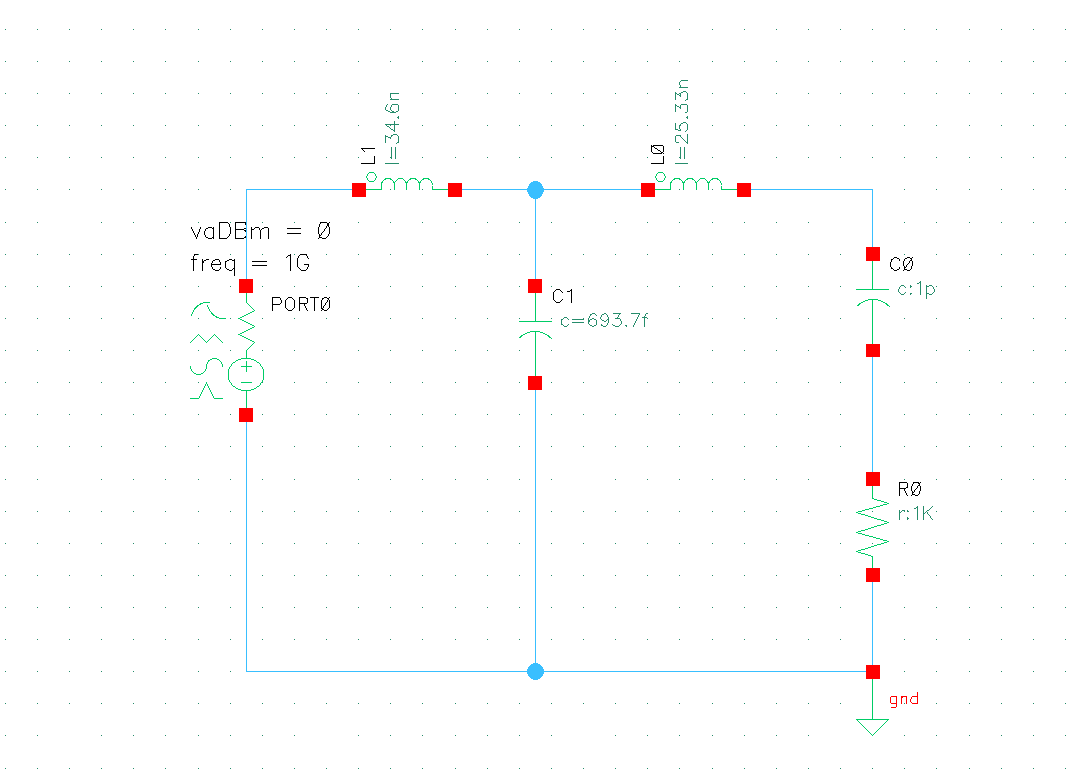
\includegraphics[width=1\linewidth]{circuit-L1.png}
      \label{fig:L1circuit}
  \end{subfigure}%
  \begin{subfigure}[t]{.4\linewidth}
    \centering
    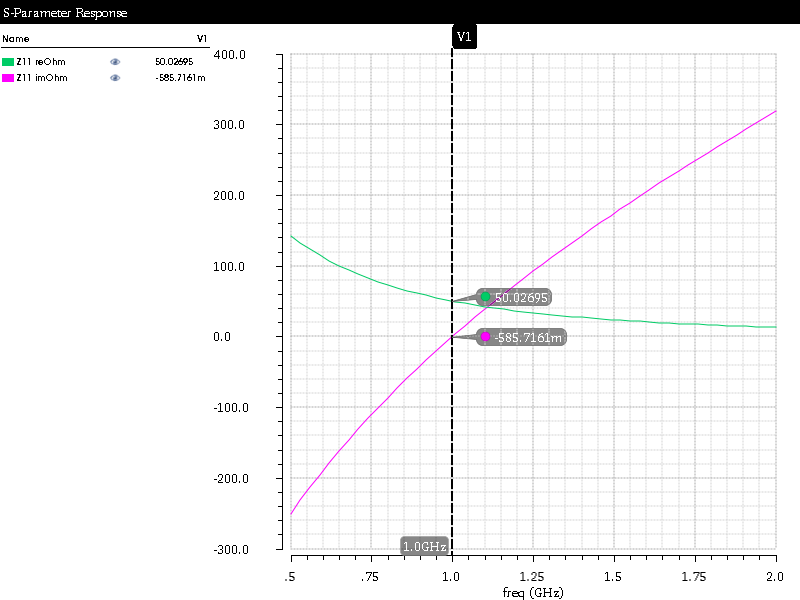
\includegraphics[width=1\linewidth]{circuit-L1-sim.png}
    \label{fig:L1circuit-sim}
  \end{subfigure}%
  \caption{Sch\'ema et Simulation du circuit}
  \label{fig:L1-sim}
\end{figure}

\subsubsection{Calcul de la tension du circuit d'adaptation}
On a :
\[
P_e = 0 \phantom{4} db_{m} = 1 mW = \frac{V^2_1}{50} \implies V_1 = \sqrt{P_0 \times 50} = 0.223 V
\]

Adaptation en puissance en $50 \Omega$, $ P_e = P_S = \frac{V^2_2}{R_0}$, sachant que $C_0$ est ''transparante'' \`a $f_0$ (r\'esonance).

\[
  V_2 = V_3 = \sqrt{R_0 \times P_e} = 1 V
\]
\begin{figure}[!htb]
  \centering
  \begin{subfigure}[t]{.5\linewidth}
      \centering
      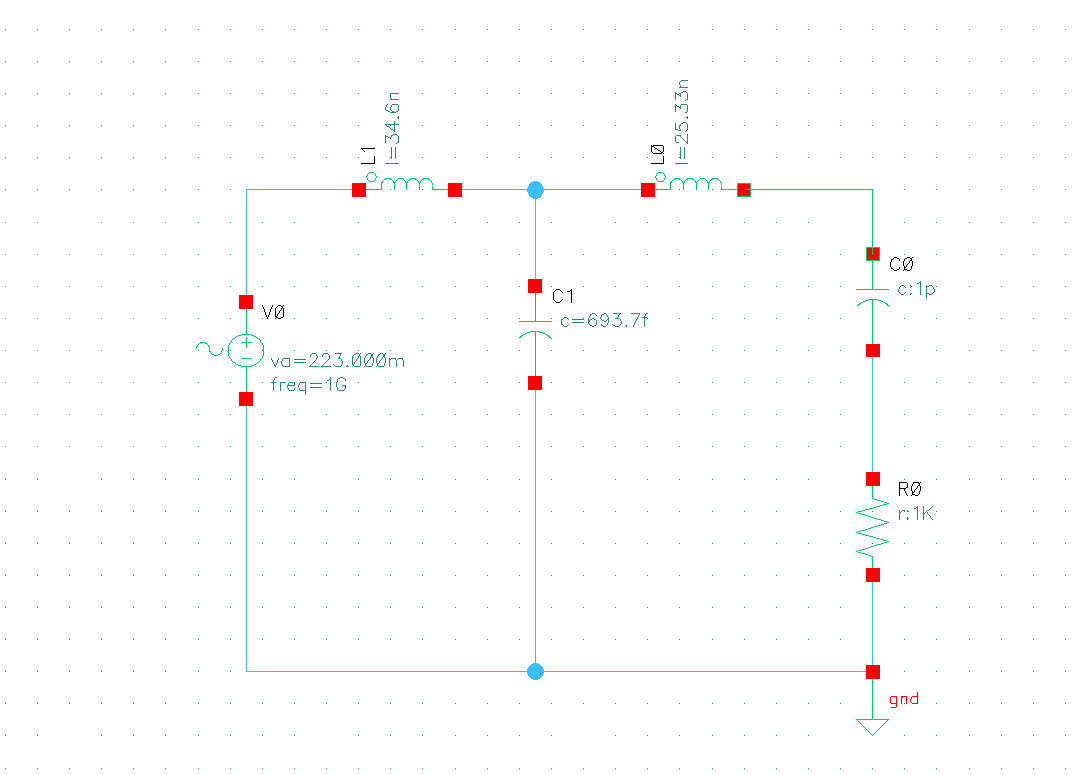
\includegraphics[width=1\linewidth]{V-Adaptation.png}
      \label{fig:Adaptation-V}
  \end{subfigure}%
  \begin{subfigure}[t]{.5\linewidth}
    \centering
    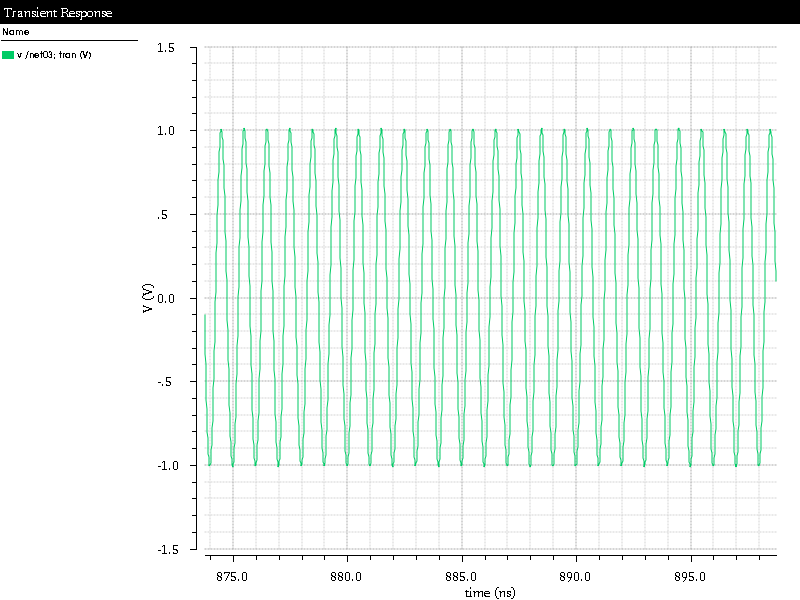
\includegraphics[width=1\linewidth]{V-Adaptation-sim.png}
    \label{fig:Adaptation-V-sim}
  \end{subfigure}%
  \caption{Sch\'ema et Simulation du circuit}
  \label{fig:Adaptation-sim}
\end{figure}

En mettant une source de tension sinuso\"idale de $V_1 = 0.223 V$ avec une r\'esistance de g\'enerateur de $50 \Omega$ \`a la place du port de
puissance $P_e$ et en faisant une simulation transient avec le r\'eseau d'adaptation calcul\'e pr\'ecedament, on retrouve une sinuso\"ide d'amplitude
1 V et de m\^eme fr\'equence aux bornes de la r\'esistance de sortie $1 K\Omega$, l'adaptation est bien v\'erifi\'e.

\clearpage

\subsection{Adaptation avec l'abaque de Smith}
\subsubsection{Principe d'adaptation avec des \'el\'ement discrets}

\begin{figure}[!htb]
\begin{center}
  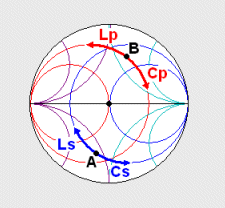
\includegraphics[scale=0.5]{adaptation_elements.png}
  \caption{Abaque repr\'esentant les adaptations avec des \'elements discrets\cite{conception-adaptation}}
\end{center}
\end{figure}

\begin{figure}[!htb]
\begin{center}
  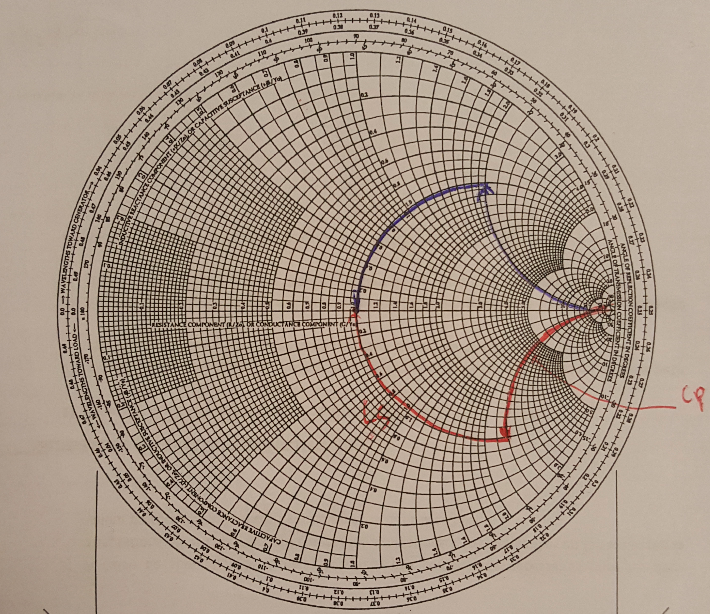
\includegraphics[scale=0.5]{adaptation_elements_proposition.png}
  \caption{Configuration selon 2 m\'ethodes possibles}
\end{center}
\end{figure}

\clearpage

\subsubsection{Adaptation avec capacit\'e parrall\`ele et inductance s\'erie}

\begin{figure}[!htb]
\begin{center}
  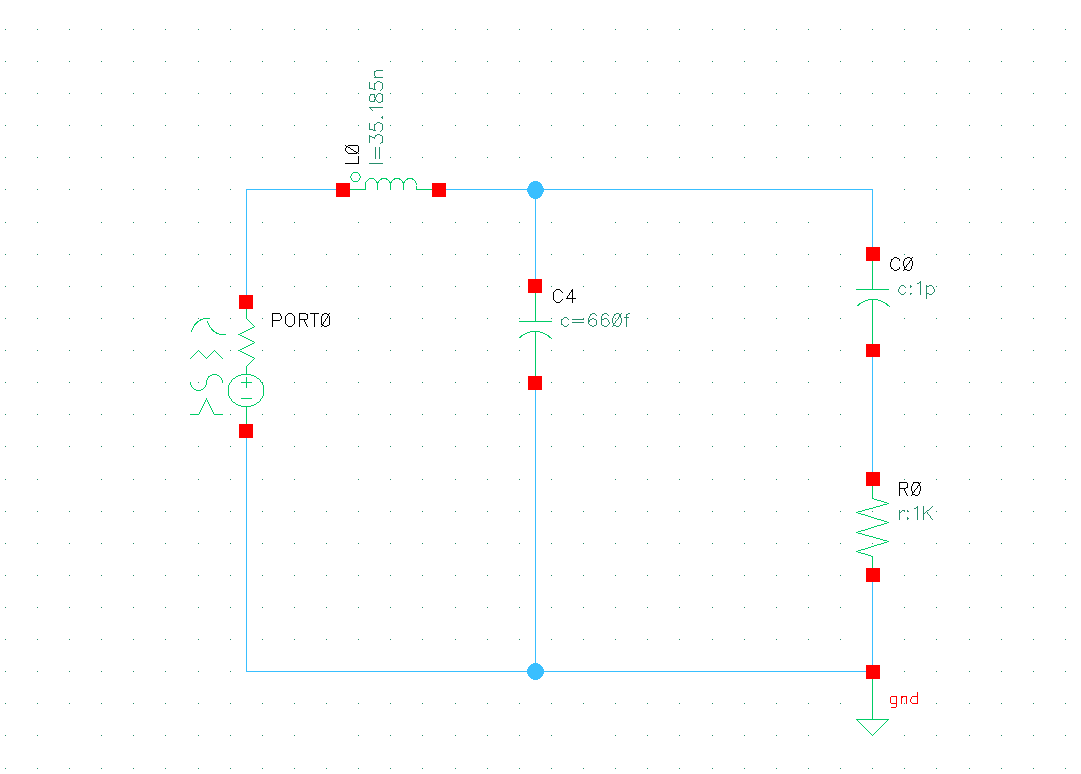
\includegraphics[scale=0.47]{architecture-Cparalle-Lseries.png}
  \caption{Sch\'ema de la premi\`ere m\'ethode d'adaptation}
\end{center}
\end{figure}

\begin{figure}[!htb]
\begin{center}
  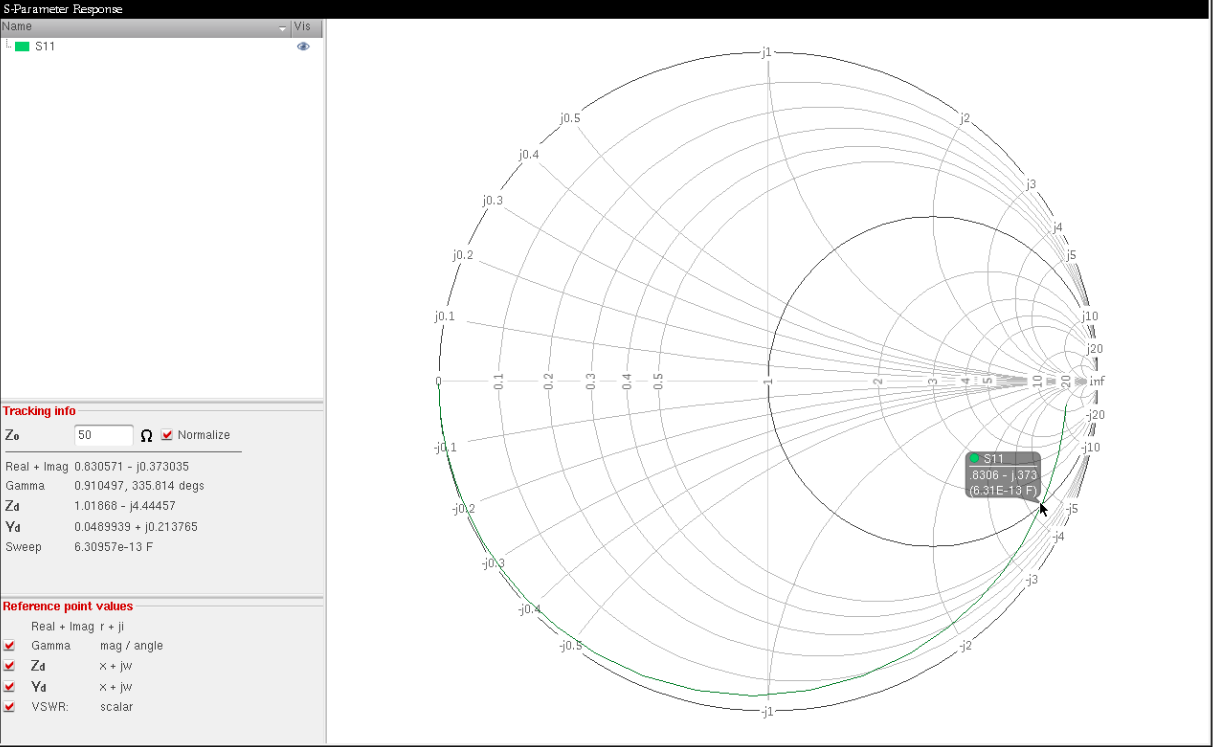
\includegraphics[width=\linewidth]{smith-capa-parallele-1st-adapt.png}
  \caption{Abaque de Smith pour une annulation de la partie imaginaire}
\end{center}
\end{figure}

\clearpage

\begin{figure}[!htb]
\begin{center}
  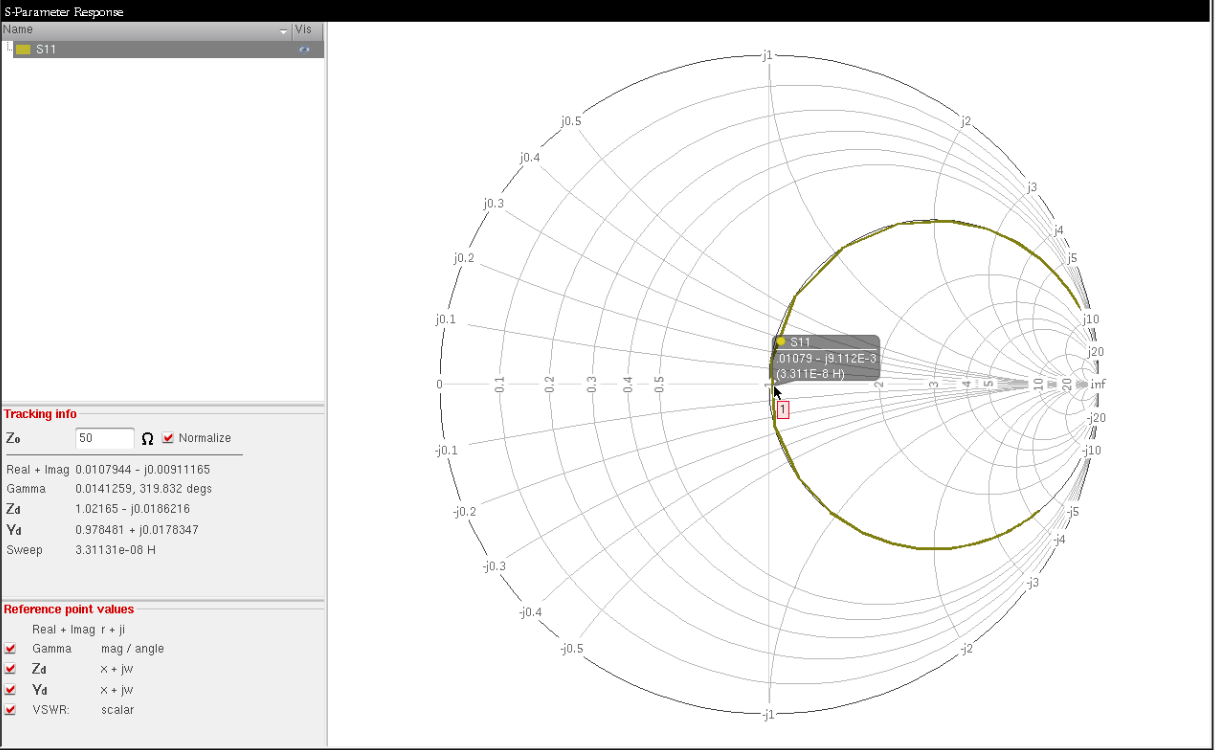
\includegraphics[width=\linewidth]{smith-induct-series-1st-adapt.png}
  \caption{Abaque de Smith repr\'esentant une adaptation compl\`ete}
\end{center}
\end{figure}

\subsubsection{Adaptation avec inductance parrall\`ele et capacit\'e s\'erie}

\begin{figure}[!htb]
\begin{center}
  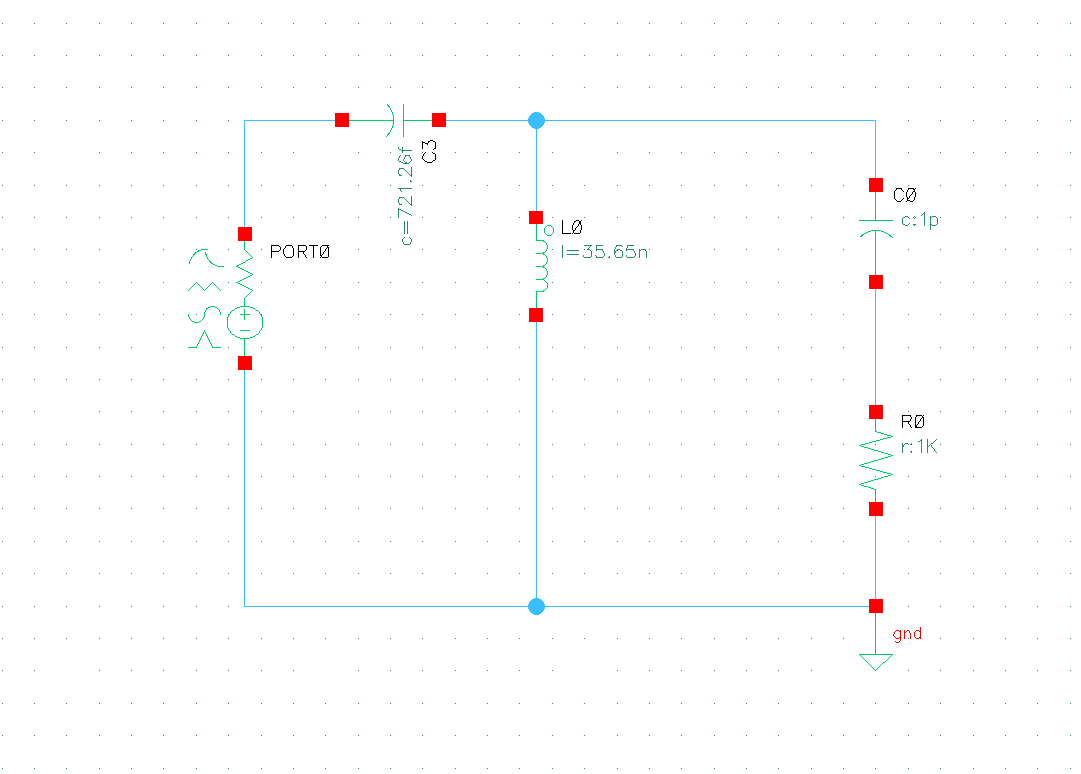
\includegraphics[scale=0.47]{architecture-Lparalle-Cseries.png}
  \caption{Sch\'ema de la deuxi\`eme m\'ethode d'adaptation}
\end{center}
\end{figure}

\clearpage

\begin{figure}[!htb]
\begin{center}
  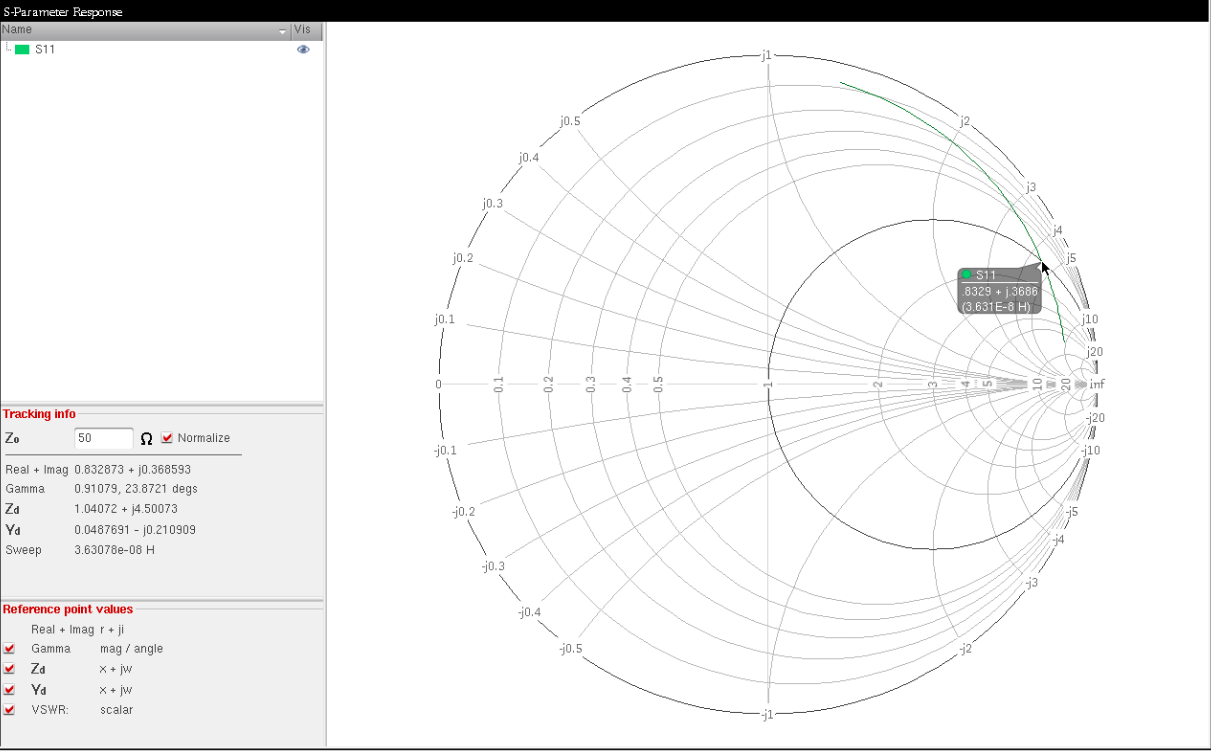
\includegraphics[width=\linewidth]{smith-induct-parallele-2nd-adapt.png}
  \caption{Abaque de Smith montrant une adaptation avec la partie imaginaire nulle}
\end{center}
\end{figure}

\begin{figure}[!htb]
\begin{center}
  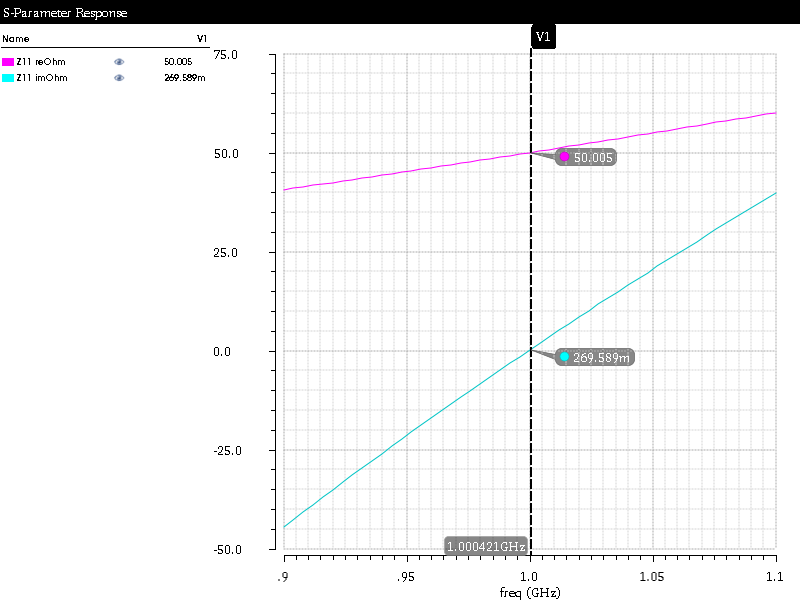
\includegraphics[scale=0.52]{Z11-2nd-adaptation.png}
  \caption{Adaptation compl\`ete apr\`es l'ajout de la capacit\'e en s\'erie}
\end{center}
\end{figure}

\clearpage

\section{Imp\'edance en entr\'ee et sortie d'un transistor}
\subsection{Mod\`ele du MOSFET petit signal}
Le mod\`ele petit signal du transistor MOSFET:

\begin{figure}[!htb]
\begin{center}
  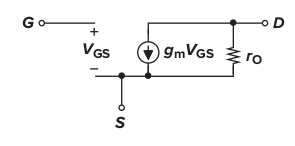
\includegraphics[scale=0.7]{MOS_small_signal.png}
  \caption{Mod\'elisation du MOSFET pour un petit signal\cite{Analog-CMOS-microelectronics} }
\end{center}
\end{figure}

\begin{figure}[!htb]
\begin{center}
  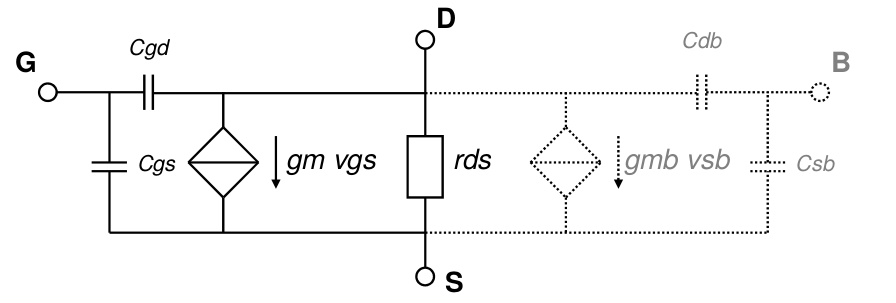
\includegraphics[scale=0.47]{complete-model.png}
  \caption{Mod\'elisation compl\`ete du MOSFET en petit signal\cite{conception-circuits-integrees}}
\end{center}
\end{figure}

\subsection{Analyse des caract\'eristiques du MOSFET avec la simulation DC}

\iffalse
\begin{wrapfigure}{r}{0.5\textwidth}
  \begin{center}
    \includegraphics[width=0.48\textwidth]{birds}
  \end{center}
  \caption{Birds}
\end{wrapfigure}
\fi

\begin{figure}[!htb]
\begin{center}
  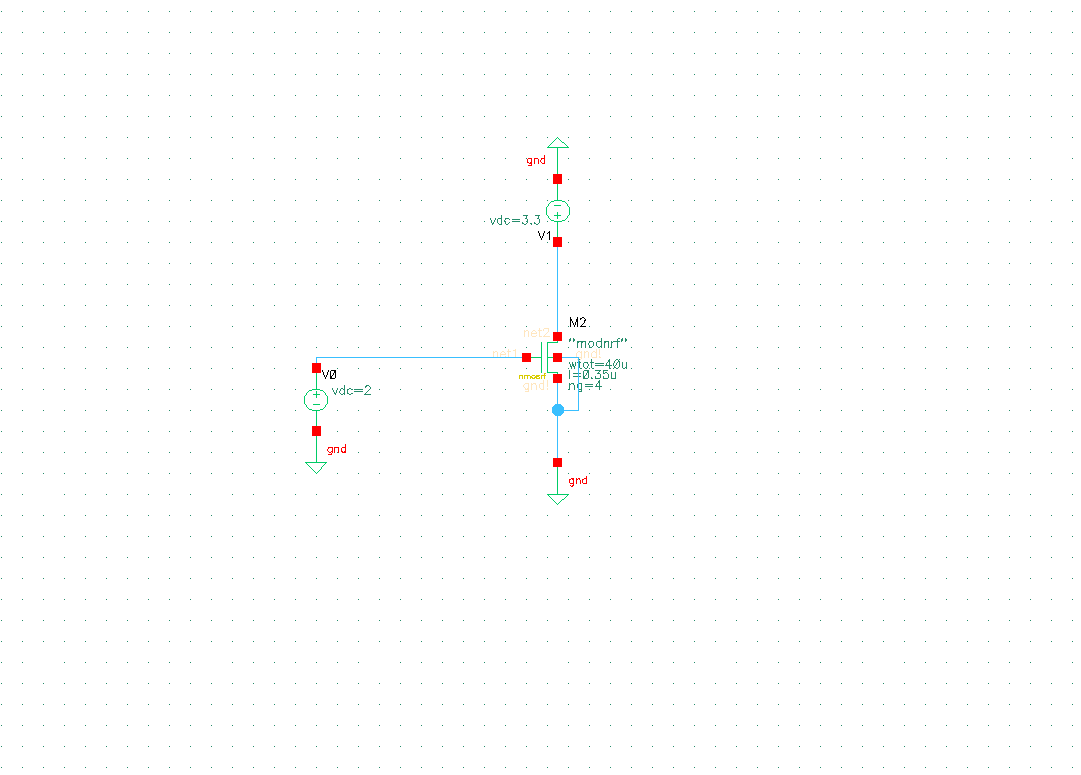
\includegraphics[scale=0.40]{arch-transistor.png}
  \caption{Sch\'ema du circuit pour une simulation DC}
\end{center}
\end{figure}

\clearpage

\begin{figure}[!htb]
\begin{center}
  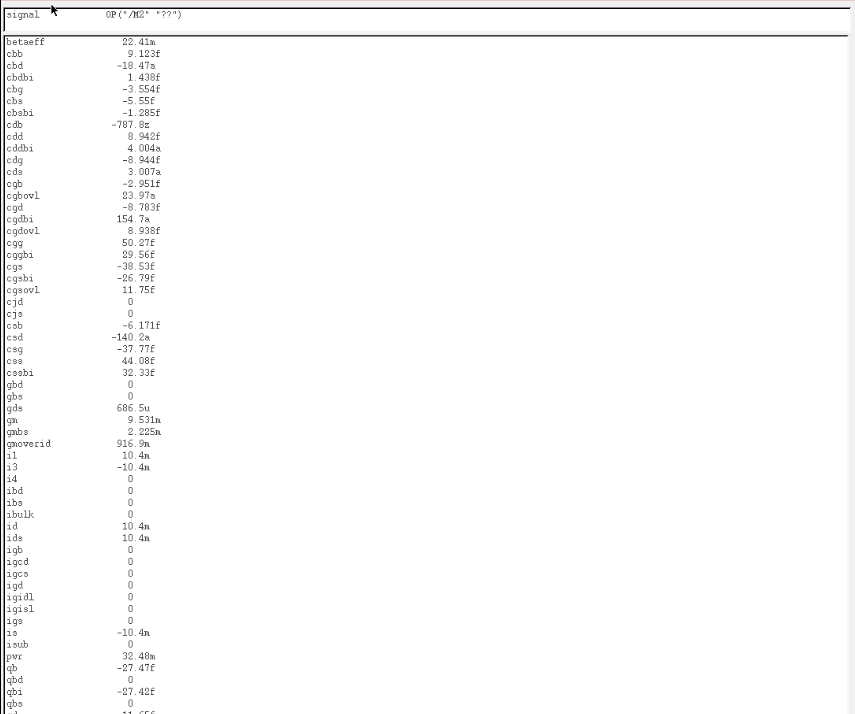
\includegraphics[scale=0.46]{Transistor-DC-1.png}
  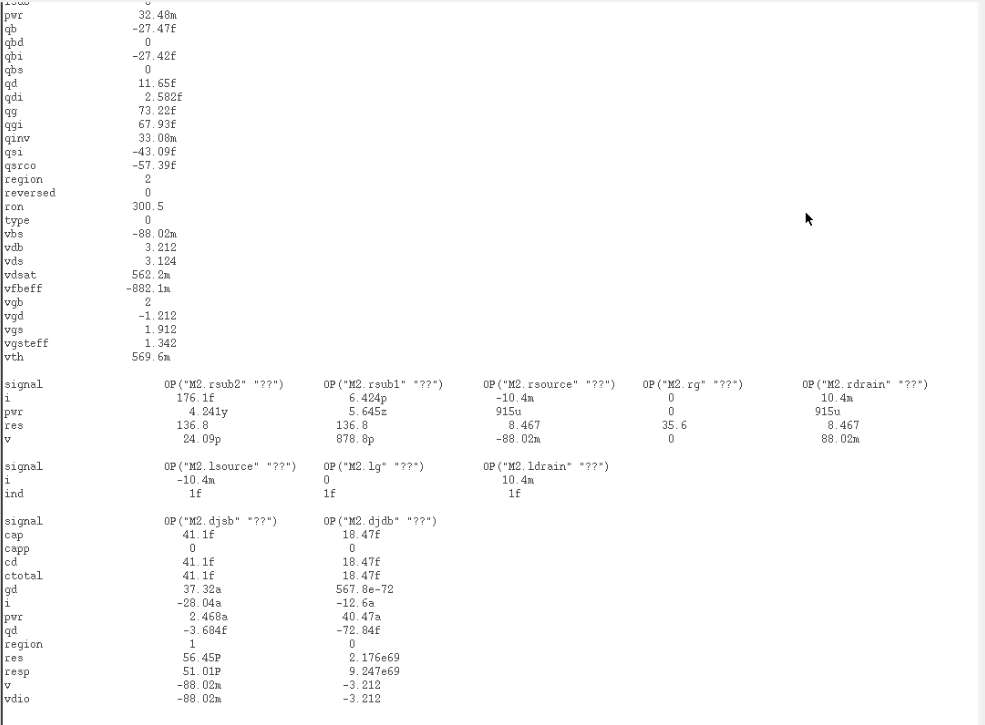
\includegraphics[scale=0.40]{Transistor-DC-2.png}
  \caption{R\'esulats de simulation DC}
\end{center}
\end{figure}

\clearpage

\subsection{Imp\'edance d'entr\'ee du MOSFET}

\begin{figure}[!htb]
\begin{center}
  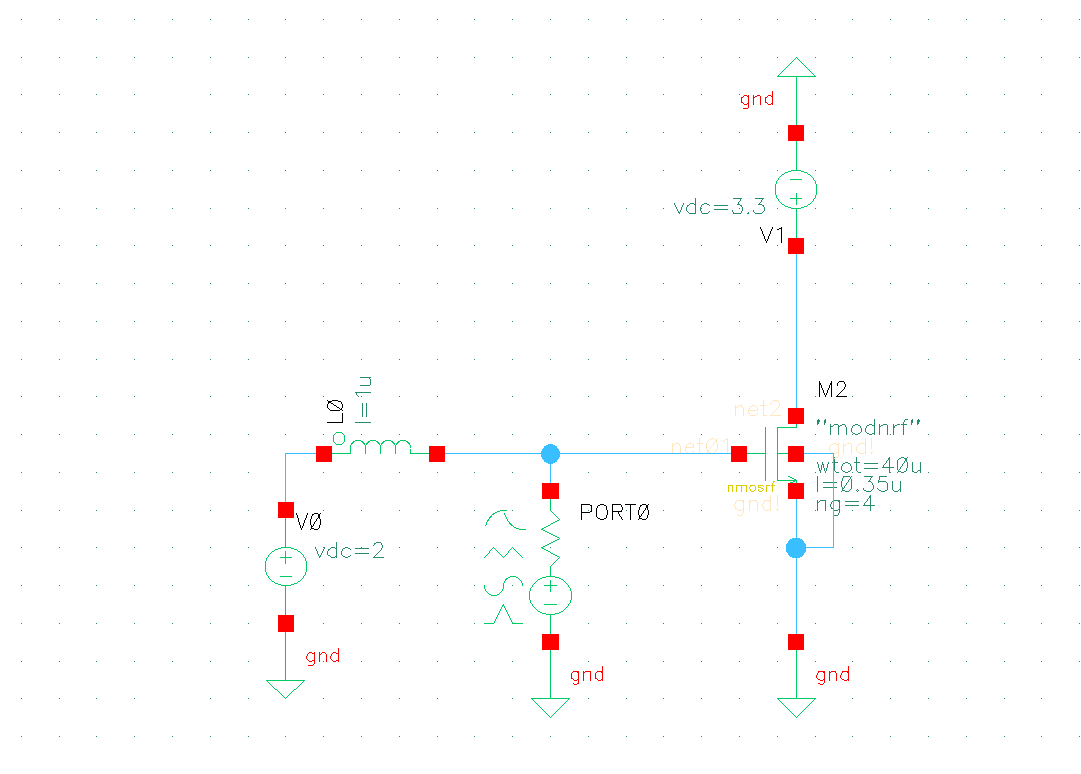
\includegraphics[scale=0.40]{arch-transistor-input-impedance.png}
  \caption{Sch\'ema du circuit pour la mesure de l'imp\'edance d'entr\'ee}
\end{center}
\end{figure}

\begin{figure}[!htb]
\begin{center}
  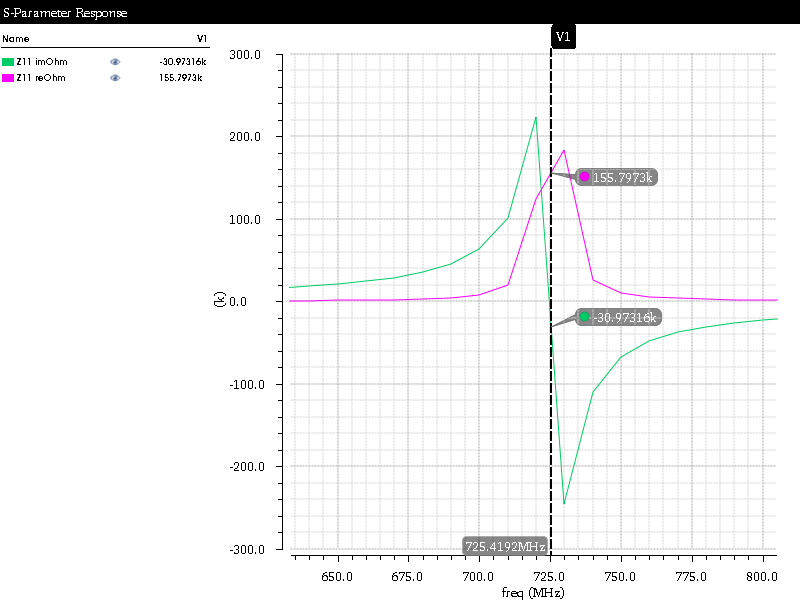
\includegraphics[scale=0.40]{sim-input-impedance.png}
  \caption{Simulation SP du param\`etre $Z_11$ en entr\'ee}
\end{center}
\end{figure}

\clearpage
\subsection{Imp\'edance en sortie du transistor}

\begin{figure}[!htb]
\begin{center}
  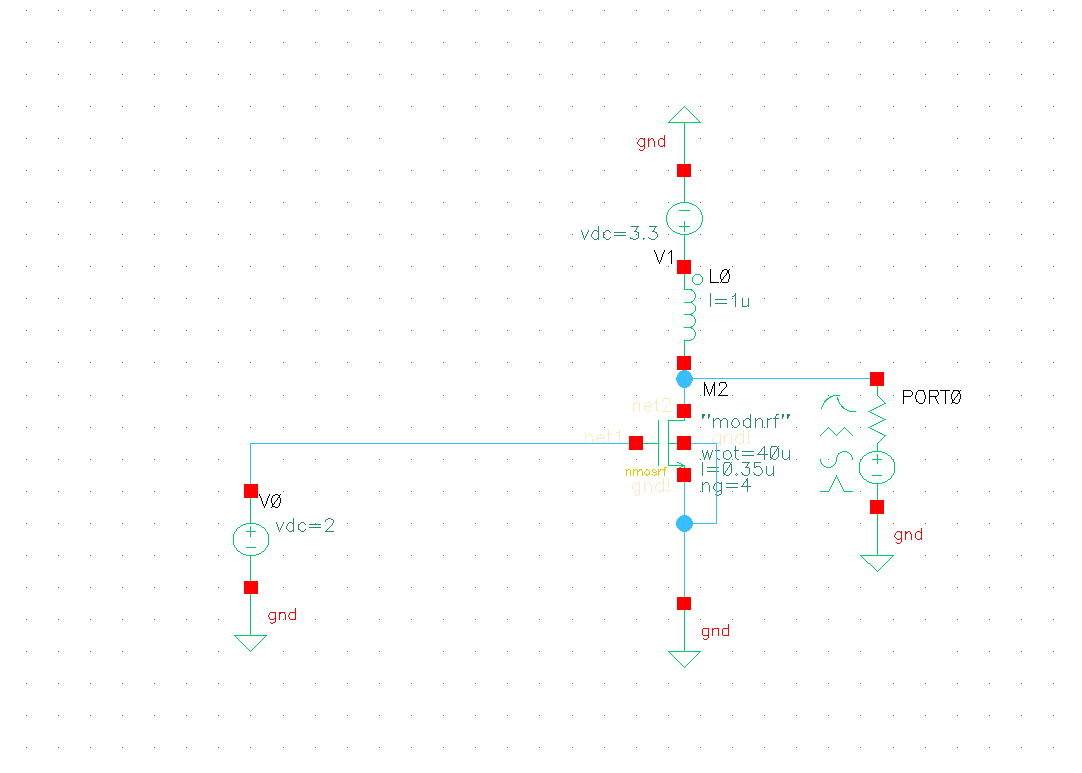
\includegraphics[scale=0.40]{arch-transistor-output-impedance.png}
  \caption{Sch\'ema du circuit pour l'imp\'edance de sortie}
\end{center}
\end{figure}

\begin{figure}[!htb]
\begin{center}
  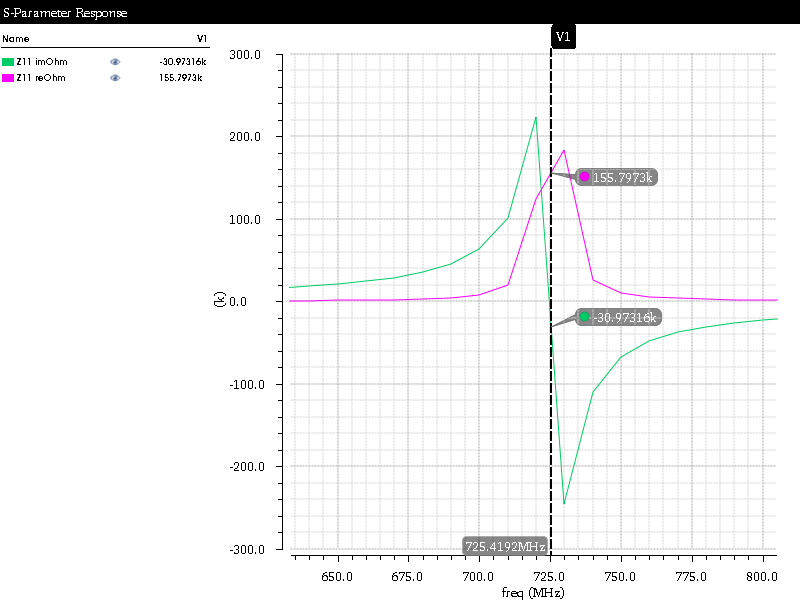
\includegraphics[scale=0.40]{sim-input-impedance.png}
  \caption{Simulation SP du param\`etre $Z_11$ sortie}
\end{center}
\end{figure}



\clearpage

\section*{Conclusion}
\addcontentsline{toc}{section}{Conclusion}


\addcontentsline{toc}{section}{R\'ef\'erences}
\begin{thebibliography}{9}

\bibitem{conception-adaptation}
\textit{Conception d'un circuit en L \`a l'aide de l'abaque de Smith}\\
\texttt{http://f5zv.pagesperso-orange.fr/RADIO/RM/RM23/RM23p/RM23p03.html}

\bibitem{Analog-CMOS-microelectronics}
\textit{Design of Analog CMOS Integrated Circuits, 2nd Edition}\\
\texttt{Behzad Razavi, McGraw-Hill Education}

\bibitem{conception-circuits-integrees}
\textit{Conception de circuits int\'egr\'es analogique}\\
\texttt{Laurent Aubard, Institut Polytechnique de Grenoble - Phelma}

\end{thebibliography}


\end{document}
